% Preamble
\documentclass[11pt,reqno,oneside,a4paper]{article}
\usepackage[a4paper,includeheadfoot,left=25mm,right=25mm,top=00mm,bottom=20mm,headheight=20mm]{geometry}
%%%% DO NOT EDIT THIS FILE

% Standard packages
\usepackage{amssymb,amsmath,amsthm}
\usepackage{xcolor,graphicx}
\usepackage{verbatim}
\usepackage{mathtools}
\usepackage{hyperref}
% Layout of headers & footers
\usepackage{titling}
\usepackage{fancyhdr}
\newcommand{\runningtitle}{Running Title}
\pagestyle{fancy} \lhead{{\theauthor}} \chead{} \rhead{{\runningtitle}} \lfoot{} \cfoot{\thepage} \rfoot{}

% Hyphenation
\hyphenation{non-zero}

% Theorem definitions in the amsthm standard
\newtheorem{thm}{Theorem}
\newtheorem{lem}[thm]{Lemma}
\newtheorem{sublem}[thm]{Sublemma}
\newtheorem{prop}[thm]{Proposition}
\newtheorem{cor}[thm]{Corollary}
\newtheorem{conc}[thm]{Conclusion}
\newtheorem{conj}[thm]{Conjecture}
\theoremstyle{definition}
\newtheorem{defn}[thm]{Definition}
\newtheorem{cond}[thm]{Condition}
\newtheorem{asm}[thm]{Assumption}
\newtheorem{ntn}[thm]{Notation}
\newtheorem{prob}[thm]{Problem}
\theoremstyle{remark}
\newtheorem{rmk}[thm]{Remark}
\newtheorem{eg}[thm]{Example}
\newtheorem*{hint}{Hint}

%% Mathmode shortcuts
% Number sets
\newcommand{\NN}{\mathbb N}              % The set of naturals
\newcommand{\NNzero}{\NN_0}              % The set of naturals including zero
\newcommand{\NNone}{\NN}                 % The set of naturals excluding zero
\newcommand{\ZZ}{\mathbb Z}              % The set of integers
\newcommand{\QQ}{\mathbb Q}              % The set of rationals
\newcommand{\RR}{\mathbb R}              % The set of reals
\newcommand{\CC}{\mathbb C}              % The set of complex numbers
\newcommand{\KK}{\mathbb K}              % An arbitrary field
% Modern typesetting for the real and imaginary parts of a complex number
\renewcommand{\Re}{\operatorname*{Re}} \renewcommand{\Im}{\operatorname*{Im}}
% Upright d for derivatives
\newcommand{\D}{\ensuremath{\,\mathrm{d}}}
% Upright i for imaginary unit
\newcommand{\ri}{\ensuremath{\mathrm{i}}}
% Upright e for exponentials
\newcommand{\re}{\ensuremath{\mathrm{e}}}
% abbreviation for \lambda
\newcommand{\la}{\ensuremath{\lambda}}
% Make epsilons look more different from the element symbol
\renewcommand{\epsilon}{\varepsilon}
% Always use slanted forms of \leq, \geq
\renewcommand{\geq}{\geqslant}
\renewcommand{\leq}{\leqslant}
% Shorthand for "if and only if" symbol
\newcommand{\Iff}{\ensuremath{\Leftrightarrow}}
% Make bold symbols for vectors
\providecommand{\BVec}[1]{\mathbf{#1}}
% Hyperbolic functions
\providecommand{\sech}{\operatorname{sech}}
\providecommand{\csch}{\operatorname{csch}}
\providecommand{\ctnh}{\operatorname{ctnh}}
% sinc function
\providecommand{\sinc}{\operatorname{sinc}}
% closure of a set
\providecommand{\clos}{\operatorname{clos}}
% The absolute value of a real number or modulus of a complex number, with automatically scaling delimiters
\newcommand{\abs}[1]{\left\lvert#1\right\rvert}
\newcommand{\sgn}{\operatorname{sgn}}

% add two sub and superscripts with a space between them
\newcommand{\Mspacer}{\;} %Spacer for below Matrix display functions
\newcommand{\M}[3]{#1_{#2\Mspacer#3}} %Print a symbol with two subscripts eg a matrix entry
\newcommand{\Msup}[4]{#1_{#2\Mspacer#3}^{#4}} %Print a symbol with two subscripts and a superscript eg a matrix entry
\newcommand{\Msups}[5]{#1_{#2\Mspacer#3}^{#4\Mspacer#5}} %Print a symbol with two subscripts and two superscripts eg a matrix entry
\newcommand{\MAll}[7]{\prescript{#1}{#2}{#3}_{#4\Mspacer#5}^{#6\Mspacer#7}} %Print a symbol with two subscripts and two superscripts eg a matrix entry

% Make really wide hat for Fourier transforms applied to large functions
\usepackage{scalerel}
\usepackage{stackengine}
\stackMath
\newcommand\reallywidecheck[1]{%
\savestack{\tmpbox}{\stretchto{%
  \scaleto{%
    \scalerel*[\widthof{\ensuremath{#1}}]{\kern-.6pt\bigwedge\kern-.6pt}%
    {\rule[-\textheight/2]{1ex}{\textheight}}%WIDTH-LIMITED BIG WEDGE
  }{\textheight}%
}{0.5ex}}%
\stackon[1pt]{#1}{\scalebox{-1}{\tmpbox}}%
}
\providecommand{\widecheck}{\reallywidecheck}

\newcommand\reallywidehat[1]{%
\savestack{\tmpbox}{\stretchto{%
  \scaleto{%
    \scalerel*[\widthof{\ensuremath{#1}}]{\kern-.6pt\bigwedge\kern-.6pt}%
    {\rule[-\textheight/2]{1ex}{\textheight}}%WIDTH-LIMITED BIG WEDGE
  }{\textheight}%
}{0.5ex}}%
\stackon[1pt]{#1}{\tmpbox}%
}


%% Acknowledgements
\newcommand{\AckYNCSRP}[1]{#1 gratefully acknowledges support from Yale-NUS College summer research programme.}
\newcommand{\AckYNCProj}[1]{#1 gratefully acknowledges support from Yale-NUS College project B grant IG18-PRB102.}
\newcommand{\AckYNCWorkshop}[1]{#1 gratefully acknowledges support from Yale-NUS College workshop grant IG18-CW003.}
\newcommand{\AckNICA}[1]{#1 would like to thank the Isaac Newton Institute for Mathematical Sciences for support and hospitality during programme \emph{Complex analysis: techniques, applications and computations}, when work on this paper was undertaken. This work was supported by EPSRC Grant Number EP/R014604/1.}
\newcommand{\AckSMRIIVP}[1]{#1 would like to thank the Sydney Mathematics Research Institute for support and hospitality under the International Visitor Programme.}
 % Standard packages, page layout, theorem environments, macros, etc
% This file contains macros specific to the project.
% You are welcome to add your own macros, but please avoid deleting those written by others.

% Asymptotic notation
\newcommand{\bigoh}{\mathcal{O}}
\newcommand{\lindecayla}{\bigoh\left(\abs{\la}^{-1}\right)}
 % Macros specific to this project.
\author{Zhang Liu}
\title{Notes on Complex Analysis}
\renewcommand{\runningtitle}{Notes on Complex Analysis}
\date{\today}

\begin{document}
\maketitle
\thispagestyle{fancy}

\begin{abstract}
    This document is to serve as a set of notes to fill the gaps in my understanding of Complex Analysis relevant to the project. This is thus not intended to be comprehensive, since only the things I am currently unfamiliar with will be included. The reference book is \textit{Complex Analysis with Applications} \cite{AG2010a}.
\end{abstract}

% \tableofcontents

\section{The Complex Field} \label{sec:ComplexField}

\begin{defn}
	A complex number $z$ is an ordered pair $(a,b)$ of real numbers. The set of all complex numbers is denoted by $\mathbb{C}$. We think of $\mathbb{C}$ as a vector space over the real numbers, and we define 
	$$1 \equiv (0,0) \text{ and } 0 \equiv (0,1).$$
	Then the set of real numbers $\mathbb{R}$ is contained in $\mathbb{C}$, and for $a,b$ real, we have the identification
	$$(a,b) = a(1,0) + b(0,1) \equiv a1+bi = a + bi.$$
\end{defn}

\par This definition is intuitively very similar to the definition of the vector space over $\mathbb{R}^2$, where $1 \equiv (0,0) \text{ and } 0 \equiv (0,1)$ are analogous to the idea of ``unit vectors," or more generally basis. This prompted me to explore the similarities and differences between the $\mathbb{R}^2$ and $\mathbb{C}$, through which my initial intuition is proven to be useful only to a limited extent and can be potentially misleading. 

A comparison between $\mathbb{R}^2$ and $\mathbb{C}$:

\begin{enumerate}
	\item The most fundamental thing is $\mathbb{R}^2$ is a vector space (over the field of real numbers), whereas $\mathbb{C}$ is a field. 
	
	\item In a vector space of $\mathbb{F}^n$, multiplication between vectors is not defined. 
	
	Recall that we define a vector space to be a set $V$ with an addition and a scalar
	multiplication on $V$. In contrast, multiplication is defined on the field of complex numbers, and so as the other algebraic properties associated with multiplication (for example, multiplicative identity, multiplicative inverse, commutativity and associativity of multiplication). 
	
	Note that the multiplicative inverse for the field of complex numbers is defined with the concept of the complex conjugate.  
	
	\item A lingering question: is the vector space $\mathbb{C}$ isomorphic to the vector space $\mathbb{R}^2$.

	This question is misleading! A vector space isomorphism is only defined between two vector spaces over the same field. $\mathbb{R}^2$ is a two dimensional field over $\mathbb{R}$ and the vector space $\mathbb{C}$ is a one dimensional vector space over field $\mathbb{C}$.
	 
	However, the field of complex numbers can be viewed as an extension field of $\mathbb{R}$ which treats $\mathbb{C}$ as a two dimensional vector space over R with basis {1, i}. 
	
	The clearest relationship between $\mathbb{C}$ and $\mathbb{R}^2$ is to say that: ``C is a two dimensional extension field of R."	(See Hungerford’s Algebra, 1974.)
	
	(The last point was retrieved from \href{https://faculty.etsu.edu/gardnerr/5510/notes/I-2.pdf}{this lecture note}.)
\end{enumerate}

\section{Cartesian Form: $z=x +iy$.}

The first way to visualize the complex numbers is to think of them as points in a Cartesian plane. This is achieved by associating each complex number $z=x +iy$ the ordered pair $(x,y)$ and then plot the point $P=(x,y).$ (hence the construction of the real axis, the imaginary axis, and the complex plane)

Some unfamiliar operations associated with the Cartesian form: 
\begin{itemize}
	\item The Absolute Value (also called norm, modulus)
	
	$$\abs{z} = \sqrt{x^2 + y^2}$$
	$$\abs{z_1 - z_2} = \sqrt{(x_1-x_2)^2 + (y_1 - y_2)^2}$$
	
	\item The Absolute Identity
	$$\abs{z} = \sqrt{z \bar{z}} \text{ or } \abs{z}^2 = z \bar{z}$$
	and its corollaries (see AG2010a \cite{AG2010a}). 
	
	\item The Absolute Inequalities
	$$\abs{\Re z} \leq \abs{z}, \abs{\Im z} \leq \abs{z};$$
	$$\abs{z} \leq \abs{\Re z} + \abs{\Im z};$$
	and the triangle inequality: 
	$$\abs{\abs{z_1}-\abs{z_2}} \leq \abs{z_1 + z_2} \leq \abs{z_1} + \abs{z_2},$$
	$$\abs{\abs{z_1}-\abs{z_2}} \leq \abs{z_1 - z_2} \leq \abs{z_1} + \abs{z_2}.$$ 
\end{itemize}

\section{Polar Form: $z = r(\cos\theta + i\sin\theta)$.}
Another useful way to visualize the complex numbers with ``rays from the origin." This is achieved by identifying a complex number with the pair $(r,\theta):$ 
\begin{itemize}
	\item $r$ is the distance from $P$ to the origin $O$, and 
	\item $\theta$ is the angle between the $x$-axis and the ray $OP$. 
\end{itemize}

We define the polar form formally: 

\begin{defn}
	Let $z=x+iy$ be a nonzero complex number. We define a number $r>0$ by setting $r = \sqrt{x^2 + y^2}>0,$ and let $\theta$ be an angle such that 
	
	$$\theta = \frac{x}{\sqrt{x^2 + y^2}} = \frac{x}{r}, \sin \theta = \frac{y}{\sqrt{x^2 + y^2}} = \frac{y}{r}.$$
	
	$r$ is called the modulus of $z$  and $\theta$ the argument of $z$. 
	
	$z = r(\cos\theta + i\sin\theta).$
\end{defn}

\subsection{Arg z and arg z} An important concept that comes with the polar form is the principle vlaue of the argument, defined as follow:
\begin{defn}
	The \textit{principle value of the argument} of a complex number $z = x+iy$ is the unique number Arg $z$ with the properties: 
	
	\begin{itemize}
		\item $-\pi < \text{Arg }z \leq \pi,$
		\item $\cos(\text{Arg }z) = \frac{x}{\abs{z}},$
		\item $\sin(\text{Arg }z) = \frac{y}{\abs{z}}.$
	\end{itemize}
	With this unique principle value defined, we can then derive the set of all values of argument: $\arg z = \{\text{Arg }z + 2k\pi: k = 0, t_1, t_2,\dots\}.$
	
\end{defn}

\subsection{Arithmetics of the Polar Form}
\begin{itemize}
	\item Multiplication.
	$$z_1 z_2 = r_1 r_2 (\cos(\theta_1 +\theta_2) + i\sin(\theta_1 +\theta_2))$$
	
	\item Division.
	$$\frac{z_1}{z_2} = \frac{r_1}{r_2} (\cos(\theta+1 - \theta_2) + i\sin(\theta_1-\theta_2))$$
\end{itemize}

\subsection{Roots of Complex Numbers}

\begin{defn}
	Let $w\neq 0$ be a complex number and $n$ a positive integer. 
	
	A number $z$ is called an nth roots of $w$ if $z^n = w$. 
\end{defn}

\begin{prop}
	(De Moivre's Identity) $(\cos \theta +i\sin \theta)^n = \cos n \theta + i\sin n \theta$.
\end{prop}

Let $w = \rho (\cos \phi + i\sin \phi) \neq 0.$ The nth roots of $w$ are the solutions of the equation $z^n= w$. These are
$$z_{k+1} = \rho^{\frac{1}{n}}(\cos(\frac{\phi}{n}+\frac{2k\pi}{n})+ i\sin(\theta_1 +\theta_2)),$$
where $k = 0,1,\dots,n-1$.

The unique number $z$ such that 
$$z^n =w \text{ and Arg }z = \frac{\text{Arg }w}{n}$$
is called the principal nth root of $w$.

The principle root is obtained by taking $\phi = \text{Arg }w$ and $k=0$. 

%Reference figures such as figure~\ref{fig:eg} as you need.
% Use this code to insert figures.
%\begin{figure}[htp]
%    \centering
    % Be sure to save all figures inside the gfx directory or they will NOT be tracked by git
%    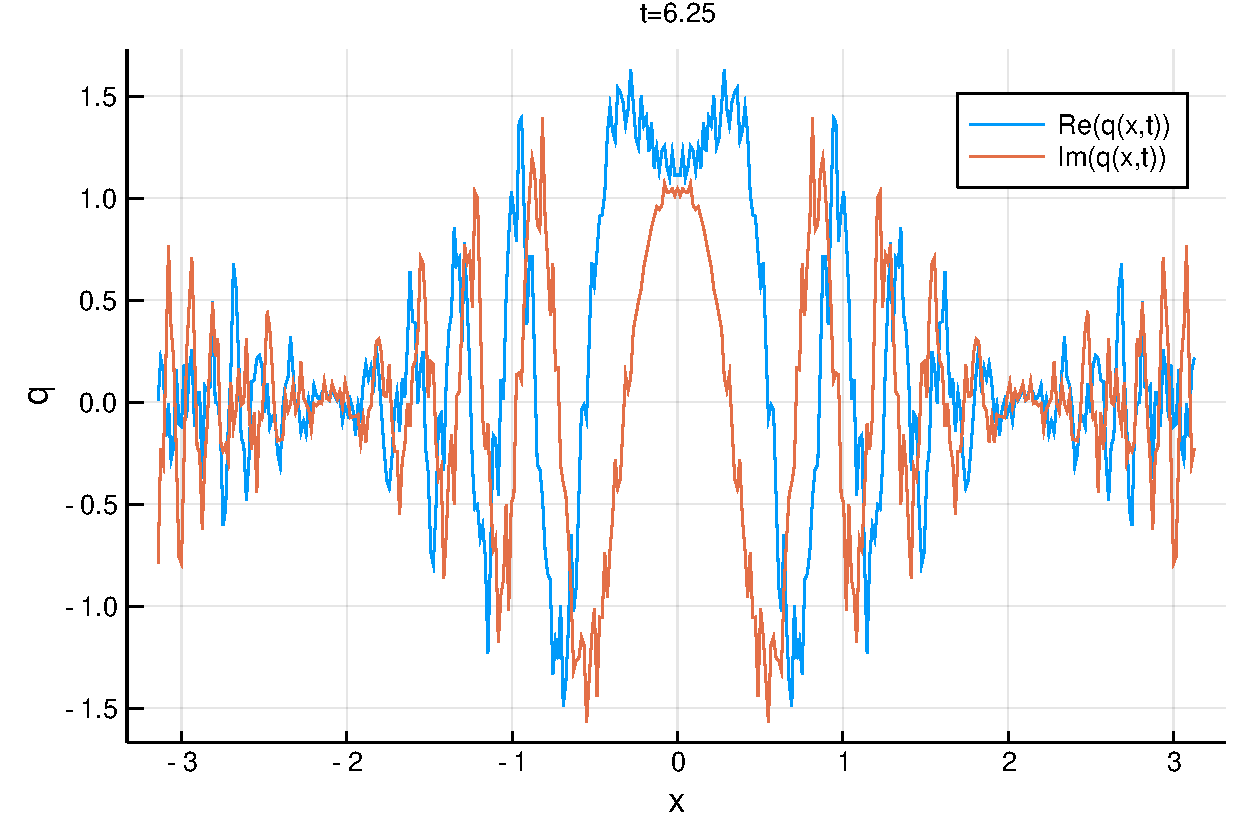
\includegraphics[width=0.8\linewidth]{gfx/fig-eg}
%    \caption{An example figure}
%    \label{fig:eg}
%\end{figure}

\bibliographystyle{amsplain}
{\small\bibliography{../dbrefs}}
\end{document}
